\documentclass[12pt]{article}
\usepackage{amsfonts, amssymb, amsmath,float,graphicx}
\parindent= 0pt
\pagestyle {empty}
\begin{document}
\section{Basic Thermodynamics}
	\subsection{Ideal Gas Equation}
		\begin{align*}
			&Ideal\;Gas\;Equation : PV = mRT = n\bar{R}T\\
			&R=\frac{\bar{R}}{M}\\
			&\bar{R} = Universal\;Gas\;Constant\\
			&M = Molecular\;mass
		\end{align*}

	\subsection{Temperature Scale conversion}
		\begin{table}[H]
			\centering
			\begin{tabular}{cc}	
				\parbox{5cm}{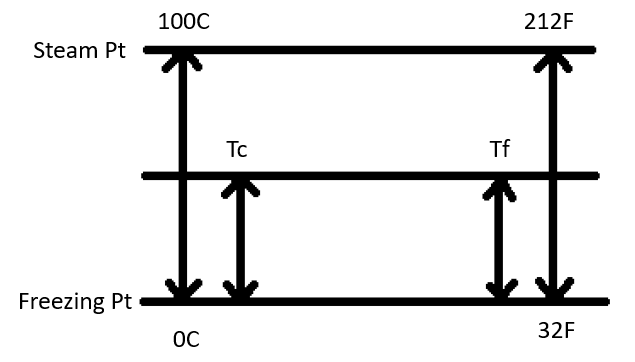
\includegraphics[scale=0.4]{TempScale.png}}& \parbox{3cm}{$\frac{t_C-0}{100-0}=\frac{t_f-32}{212-32}$}
			\end{tabular}
		\end{table}
				
			
\section{Fixed Mass Energy analysis}
	\begin{table}[H]
		\centering
		\begin{tabular}{cc}
			\parbox{5cm}{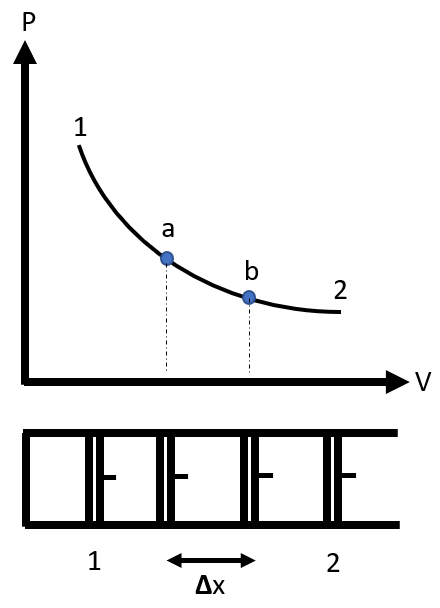
\includegraphics[scale=0.5]{closedsyswork.png}} 
			& \parbox{7cm}{
			\begin{align*}
			Work(W)&= Force(F)*distance(\partial x)\\
			&= PA\partial x\\
			&= P\partial v\\
			&= PdV\\
			\boxed{W = \int PdV}
			\end{align*}
			The above work is called Non-flow work or closed system work or boundary work}
		\end{tabular}
	\end{table}
	
	\subsection{Work formulae for various processes}
		$\textbf{Constant\;Volume\;work}: W = \int PdV = 0$\\
		$\textbf{Constant\;Pressure\;work}: W = \int \limits_1^2 PdV = \boxed{P(V_2-V_1)}$\\
		$\textbf{Constant\;Temperature\;work}:$
		\begin{equation} W = \int PdV
		\end{equation}
		For Ideal gas, $PV=mRT$. Here \textbf{mRT} is constant since T is constant in Isothermal process and \textbf{m} and \textbf{R} are already constants.\\\\
		\begin{equation}
		PV = C
		\end{equation}	
 		$\implies P = \dfrac{C}{V}\;\;or\;\;V = \dfrac{C}{P}.\quad Use\;P = \dfrac{C}{V}\;in\;(1)$\\\\
		$\implies W = \int\limits_1^2\dfrac{C}{V}\,dV = \boxed{C\ln\dfrac{V_2}{V_1}}$\\\\
		From $(2),\;\dfrac{V_2}{V_1} = \dfrac{P_1}{P_2} \implies \boxed{W = C\dfrac{P_1}{P_2}}$
		
		
		
\end{document}
